% !TeX root = ../tfg.tex
% !TeX encoding = utf8

\chapter{Fundamentos matemáticos del aprendizaje profundo} \label{chap:dl-mates}
Posteriormente, después de haber sentado las bases del aprendizaje automático, vamos a profundizar en las redes neuronales artificiales y en el aprendizaje profundo como aproximación avanzada capaz de modelar funciones complejas. Se explicarán los fundamentos matemáticos necesarios para su entrenamiento, incluidos los algoritmos de optimización basados en gradiente y el algoritmo de retropropagación. Finalmente, se discutirán aspectos avanzados como la selección de funciones de coste, tipos de unidades de salida y ocultas, así como conceptos de transferencia de aprendizaje y redes neuronales convolucionales, incluyendo las operaciones de convolución y pooling.

Aunque los algoritmos clásicos de aprendizaje automático han demostrado ser eficaces en muchos problemas relevantes, no han sido capaces de abordar con éxito algunos de los grandes retos de la inteligencia artificial, como el reconocimiento de voz o la identificación automática de objetos en imágenes. Uno de los principales motivos es la dificultad para generalizar correctamente cuando se trabaja con datos de alta dimensión, donde los métodos tradicionales suelen fallar o requerir un esfuerzo computacional elevado. Además, las técnicas clásicas carecen de la capacidad de representar funciones complejas necesarias en estos entornos. En respuesta a estas limitaciones, surge el aprendizaje profundo (deep learning), una rama del aprendizaje automático que introduce arquitecturas más potentes y mecanismos adaptativos con el objetivo de aprender representaciones útiles y eficaces incluso en espacios de gran complejidad.

Una red neuronal artificial (RNA) se inspira en la estructura de las redes neuronales del cerebro \parencite{Goodfellow-et-al-2016}. Una RNA consiste en un conjunto de funciones elementales conectadas entre sí, donde cada función procesa entradas y transmite una salida a otras unidades. Estas redes se estructuran como grafos dirigidos acíclicos, donde los nodos representan neuronas y las aristas conexiones con pesos asociados. Una red neuronal define una función $y = f(x; \theta)$ que aprende los parámetros $\theta$ para busca aproximar una función objetivo $f^*$, utilizando una sucesión de transformaciones funcionales compuestas. Esta composición se puede expresar como:

\begin{equation}
f(x) = f^{(L)}(f^{(L-1)}(\dots f^{(1)}(x)))
\end{equation}

Su estructura se define por capas de unidades (\textit{neuronas}) interconectadas. En la Figura \ref{fig:red-neuronal} tenemos un ejemplo de una red neuronal feedfoward. La longitud de la cadena determina la \textit{profundidad} del modelo, de ahí el término \textit{aprendizaje profundo} o \textit{deep learning}:
\begin{itemize}
    \item \textbf{Capa de entrada}: Recibe los valores iniciales de $\mathbf{x}$. Son las capas más situadas a la izquierda en que se encuentran las neuronas de entrada, las cuales se encargan de percibir los datos recibidos a través de las entradas.
    \item \textbf{Capas ocultas}: Son capas intermedias de neuronas. El comportamiento de estas capas no está especificado por los datos. El algoritmo de aprendizaje debe decidir cómo utilizar estas capas para producir la salida deseada, pero los datos no indican qué debe hacer cada capa individual. Por tanto, el algoritmo debe encontrar la mejor manera de usar estas capas para aproximar la función $f^*$.
    \item \textbf{Capa de salida}: Son las capas más situadas a la derecha. Produce el resultado final de la red. Si la salida es un valor continuo (regresión), puede usarse una función de activación lineal o sigmoide. Para clasificación, se suelen usar funciones como softmax para probabilidades multinomiales.
\end{itemize}

Durante el entrenamiento de una red neuronal, se busca que la función aprendida $f(x)$ se aproxime a una función objetivo $f^*(x)$. Los datos de entrenamiento nos proporcionan ejemplos aproximados de $f^*(x)$ evaluados en distintos puntos. Cada ejemplo $x$ está asociado a una etiqueta $y \approx f^*(x)$.


\begin{figure}[!htbp]
    \centering
    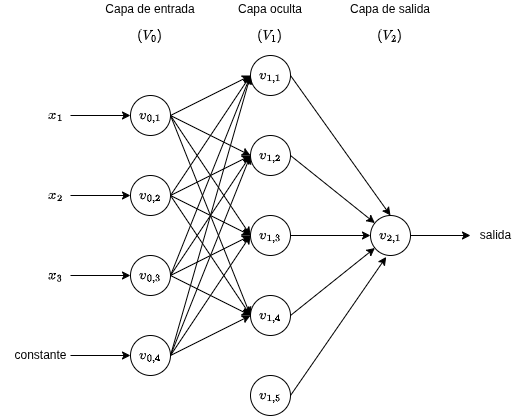
\includegraphics[width=0.8\textwidth]{img/red_neuronal.png}
    \caption{Red neuronal feedforward en capas de profundidad 2, tamaño 10 y anchura 5. Hay una neurona en la capa oculta que no tiene aristas entrantes. Además, hay una neurona en la capa oculta que no tiene aristas entrantes. La salida de esta neurona será $f^{(1)}(0)$, es decir, la función de activación evaluada en $0$. Elaboración propia. }
    \label{fig:red-neuronal}
\end{figure}


Una forma de entender el papel de las redes neuronales es partir de las limitaciones de los modelos lineales clásicos, como la regresión lineal o logística. Estos modelos son muy útiles por su simplicidad y eficiencia, pero tienen un problema fundamental: solo pueden capturar relaciones lineales entre las variables de entrada, lo que limita su capacidad para modelar fenómenos complejos del mundo real.

Para superar esta limitación, la idea es aplicar el modelo lineal no directamente sobre la entrada original \(x\), sino sobre una transformación no lineal de los datos, denotada por \(\phi(x)\). Así, en lugar de aprender una función lineal en el espacio original, se aprende una función lineal en un espacio transformado donde las relaciones sean más sencillas de modelar. El problema entonces se convierte en decidir qué transformación no lineal \(\phi\) usar.

Existen varios enfoques para definir esta transformación:

\begin{itemize}
    \item \textbf{Diseñar manualmente \(\phi\)}: consiste en especificar de forma experta qué transformaciones aplicar en función del problema concreto. Este era el enfoque tradicional antes del \textit{deep learning}, pero tiene la desventaja de requerir mucho conocimiento experto y no ser fácilmente reutilizable entre dominios distintos.
    
    \item \textbf{Usar transformaciones muy generales de alta dimensión}: se pueden usar transformaciones genéricas con suficiente flexibilidad para ajustar cualquier patrón en los datos de entrenamiento. Sin embargo, esto suele conllevar un alto riesgo de sobreajuste y mala capacidad de generalización a datos nuevos.
    
    \item \textbf{Aprender automáticamente \(\phi\) a partir de los datos}: esta es la idea central del \textit{deep learning}. Aquí se parametriza \(\phi\) mediante un conjunto de parámetros \(\theta\), que se aprenden directamente del conjunto de datos. El modelo resultante se puede escribir como:
    \[
    y = f(x; \theta, w) = \phi(x; \theta)^\top w,
    \]
    donde \(\theta\) define la transformación no lineal aprendida y \(w\) los pesos de la capa de salida. Aunque esta aproximación elimina la simplicidad y convexidad de los modelos lineales, ofrece la gran ventaja de aprender representaciones adaptadas automáticamente a la tarea.
\end{itemize}

El enfoque del \textit{deep learning} consiste precisamente en aprender estas transformaciones intermedias de forma jerárquica y a gran escala, optimizando todas las capas de la red simultáneamente a partir de los datos. Esto permite descubrir representaciones intermedias que capturan estructuras relevantes del problema, ofreciendo un marco matemático flexible y potente para abordar tareas como clasificación, regresión, segmentación y más.

\section{Aprendizaje de las redes neuronales}
El diseño y entrenamiento de una red neuronal no difiere demasiado del entrenamiento de otros modelos de aprendizaje automático basados en descenso por gradiente. La principal diferencia entre los modelos lineales y las redes neuronales radica en que la no linealidad de estas últimas hace que la mayoría de las funciones de pérdida interesantes sean no convexas. Esto implica que las redes neuronales suelen entrenarse mediante algoritmos iterativos basados en el gradiente, que buscan reducir la función de coste a un valor bajo, en lugar de utilizar métodos analíticos como los empleados en la regresión lineal o técnicas de optimización convexa, como las usadas en regresión logística o máquinas de vectores soporte (SVM), que sí tienen garantías de convergencia global. 

El descenso de gradiente estocástico aplicado a funciones de pérdida no convexas no tiene garantía de convergencia, y es sensible a los valores de los parámetros iniciales. Para las redes neuronales feedforward, es importante inicializar todos los pesos con valores aleatorios pequeños.


\section{Procesos de propagación}

\subsection{Propagación hacia Adelante}

En una red neuronal feedforward, la entrada $\mathbf{x}$ se transforma capa a capa hasta producir la salida $\hat{y}$ mediante un proceso llamado \emph{propagación hacia adelante}:

\[
\hat{y} = f(\mathbf{x}; \theta).
\]

Durante entrenamiento, este flujo se extiende hasta obtener un coste escalar:

\[
J(\theta) = L(\hat{y}, y) + \Omega(\theta),
\]

donde $L$ es la función de pérdida, $\Omega$ es un término de regularización, $y$ y es la etiqueta verdadera e $\hat{y}$ es la predicción de la red neuronal.

\subsection{Algoritmo de Back-Propagation}

El objetivo del entrenamiento es minimizar $J(\theta)$. Para ello necesitamos su gradiente respecto a los parámetros $\theta$:

\[
\nabla_\theta J(\theta).
\]

El \emph{algoritmo de back-propagation}, introducido por \cite{rumelhart1986learning}, permite calcular este gradiente de manera eficiente aplicando sistemáticamente la regla de la cadena a través del grafo computacional de la red. Es importante aclarar que back-propagation no constituye el algoritmo de aprendizaje completo, ya que únicamente calcula los gradientes, mientras que el ajuste de los parámetros se realiza con otro método, como por ejemplo el gradiente descendente estocástico. Además, back-propagation no es exclusivo de las redes neuronales, ya que puede aplicarse a cualquier función diferenciable representada como un grafo computacional. 

Para formalizar este concepto, representamos la red como un grafo dirigido acíclico (DAG) donde cada nodo $u^{(i)}$ corresponde a una variable (que puede ser un escalar, vector o tensor) calculada mediante una operación:

\[
u^{(i)} = f^{(i)}(A^{(i)}),
\]

donde $A^{(i)}$ es el conjunto de nodos padre o entradas de la operación. 

En este contexto, la regla de la cadena del cálculo diferencial se utiliza para calcular derivadas de funciones compuestas a partir de las derivadas de funciones más simples. La retropropagación es un algoritmo que calcula la regla de la cadena, con un orden específico de operaciones que resulta muy eficiente.

Sea $x \in \mathbb{R}$, y sean $f$ y $g$ funciones $f,g: \mathbb{R} \to \mathbb{R}$. Supongamos que $y = g(x)$ y $z = f(g(x)) = f(y)$. Entonces, la regla de la cadena establece que
\[
\frac{dz}{dx} = \frac{dz}{dy} \frac{dy}{dx}.
\]
Podemos generalizar esto más allá del caso escalar. Supongamos que $x \in \mathbb{R}^m$, $y \in \mathbb{R}^n$, $g:\mathbb{R}^m \to \mathbb{R}^n$, y $f:\mathbb{R}^n \to \mathbb{R}$. Si $y = g(x)$ y $z = f(y)$, entonces

\[
\frac{\partial z}{\partial x_i} = \sum_j \frac{\partial z}{\partial y_j} \frac{\partial y_j}{\partial x_i}. \tag{6.45}
\]

En notación vectorial, esto puede escribirse de forma equivalente como

\[
\nabla_x z = J_g(x)^\top \nabla_y z,
\]

donde $J_g(x)$ es la matriz Jacobiana $n \times m$ de $g$ evaluada en $x$.

\vspace{0.3cm}

De esto vemos que el gradiente de una variable $\mathbf{x}$ se puede obtener multiplicando una matriz Jacobiana $J_g(x)$ por un gradiente $\nabla_y z$. El algoritmo de retropropagación consiste en realizar exactamente este producto Jacobiano-gradiente para cada operación en el grafo.

\vspace{0.3cm}

Usualmente no aplicamos el algoritmo de retropropagación únicamente a vectores, sino a tensores de dimensionalidad arbitraria. Conceptualmente, esto es exactamente lo mismo que la retropropagación con vectores. La única diferencia es cómo están organizados los números en una cuadrícula para formar un tensor. Podemos imaginar aplanar cada tensor en un vector antes de ejecutar la retropropagación, computar un gradiente con valores vectoriales y luego volver a darle forma de tensor al gradiente. En esta forma reorganizada, la retropropagación sigue siendo simplemente multiplicar Jacobianas por gradientes.

\vspace{0.3cm}

Para denotar el gradiente de un valor $z$ con respecto a un tensor $\mathbf{X}$, escribimos $\nabla_{\mathbf{X}} z$, igual que si $\mathbf{X}$ fuera un vector. Los índices dentro de $\mathbf{X}$ ahora tienen múltiples coordenadas, por ejemplo, un tensor 3-D está indexado por tres coordenadas. Podemos abstraer esto usando un solo índice $i$ para representar el conjunto completo de índices. Para todos los posibles índices $i$, $(\nabla_{\mathbf{X}} z)_i$ da $\frac{\partial z}{\partial X_i}$. Esto es exactamente lo mismo que para todos los posibles índices enteros en un vector, $(\nabla_x z)_i$ da $\frac{\partial z}{\partial x_i}$. Usando esta notación, podemos escribir la regla de la cadena tal como se aplica a tensores. Si $Y = g(\mathbf{X})$ y $z = f(Y)$, entonces

\[
\nabla_{\mathbf{X}} z = \sum_j (\nabla_Y z)_j \frac{\partial Y_j}{\partial \mathbf{X}_i}. \tag{6.47}
\]

El algoritmo general de Back-Propagation puede describirse de la siguiente manera: 

Sea $u^{(n)}$ la salida escalar final, queremos calcular $\frac{\partial u^{(n)}}{\partial u^{(j)}}$ para cada nodo intermedio $u^{(j)}$. Denotamos por $u^{(i)}$ a los nodos hijos directos de $u^{(j)}$ en el grafo computacional, es decir, aquellos que dependen directamente de $u^{(j)}$. La fórmula recursiva es:

\[
\frac{\partial u^{(n)}}{\partial u^{(j)}} = \sum_{i : j \in \text{Pa}(u^{(i)})} \frac{\partial u^{(n)}}{\partial u^{(i)}} \frac{\partial u^{(i)}}{\partial u^{(j)}},
\]

donde el conjunto $\text{Pa}(u^{(i)})$ representa los padres de $u^{(i)}$ en el grafo; la condición $j \in \text{Pa}(u^{(i)})$ significa que $u^{(i)}$ depende directamente de $u^{(j)}$.

Vamos a describir el pseudocódigo simplificado del algoritmo general explicado:

\begin{enumerate}
    \item Ejecutar propagación hacia adelante para obtener todos los $u^{(i)}$.
    \item Inicializar $\text{grad}[u^{(n)}] \gets 1$.
    \item Para $j = n-1$ hasta $1$:
    \[
    \text{grad}[u^{(j)}] \gets \sum_{i: j \in \text{Pa}(u^{(i)})} \text{grad}[u^{(i)}] \frac{\partial u^{(i)}}{\partial u^{(j)}}.
    \]
\end{enumerate}



Las ventajas computacionales de este algoritmo son: 
\begin{itemize}
    \item \textbf{Eficiencia}: evita recalcular subexpresiones compartidas, reduciendo costo de $O(\exp(n))$ a $O(n)$ en grafos en cadena.
    \item  \textbf{Memoria}: guarda activaciones necesarias para el backward pass.
    \item \textbf{Generalidad}: soporta operaciones arbitrarias (matrices, tensores, etc.).
\end{itemize}

\section{Función de coste}
Un aspecto clave en el diseño de una red neuronal profunda es la elección de la función de coste. Afortunadamente, estas funciones suelen ser bastante similares a las utilizadas en otros modelos paramétricos, como los modelos lineales.

En la mayoría de los casos, el modelo paramétrico define una distribución de probabilidad $p(y \mid x; \theta)$, y aplicamos el principio de máxima verosimilitud. Esto se traduce en el uso de la \textit{entropía cruzada} entre los datos de entrenamiento y las predicciones del modelo como función de coste.

En algunas situaciones, se opta por un enfoque más sencillo: en lugar de estimar la distribución completa de $y$ dado $x$, se predice solo una estadística de $y$ condicionada a $x$. Para ello, se emplean funciones de pérdida especializadas que permiten entrenar al modelo como estimador de dicha cantidad.

La función de coste total utilizada para entrenar una red neuronal suele ser la combinación de una de estas funciones de coste principales con un término de regularización, como por ejemplo la técnica de \textit{weight decay}.

\section{Unidades de salida}
La elección de la función de coste está muy ligada al tipo de unidad de salida utilizada. En la mayoría de los casos, se emplea la entropía cruzada entre la distribución de los datos y la distribución estimada por el modelo. La forma concreta de la función de entropía cruzada depende de cómo se representen las salidas del modelo.

Cualquier tipo de unidad neuronal que se use como salida también puede emplearse como unidad oculta. A continuación, supondremos que la red feedforward genera un conjunto de características ocultas $h = f(x; \theta)$. La capa de salida transforma estas características para completar la tarea que debe realizar la red.

\subsection{Unidades lineales}

Un tipo simple de unidad de salida es la unidad lineal, que aplica una transformación afín sin función de activación no lineal. Dado un vector de características $h$, la salida se calcula como:
\[
\hat{y} = W^\top h + b
\]
Estas unidades se utilizan frecuentemente para predecir la media de una distribución Gaussiana condicional:
\[
p(y \mid x) = \mathcal{N}(y; \hat{y}, I)
\]
Maximizar la log-verosimilitud en este caso equivale a minimizar el error cuadrático medio (MSE).

El marco de máxima verosimilitud también permite modelar la covarianza de la Gaussiana, incluso hacerla dependiente de la entrada. Sin embargo, asegurar que esta covarianza sea una matriz definida positiva para cualquier entrada resulta difícil usando solo una capa lineal. Por ello, se emplean unidades de salida más sofisticadas para parametrizar la covarianza.

Dado que las unidades lineales no saturan, son compatibles con algoritmos de optimización basados en gradientes y se pueden usar con diversos métodos de optimización.

\subsection{Unidades sigmoidales}

Muchas tareas requieren predecir una variable binaria $y$, de hecho, el problema abordado será de este tipo, es decir, un problema de clasificación con dos clases, se pueden plantear de este modo. El enfoque de máxima verosimilitud define una distribución Bernoulli condicional:
\[
p(y \mid x) = \text{Bernoulli}(y; \hat{y})
\]
En este caso, la red necesita predecir solamente la probabilidad $P(y = 1 \mid x)$, la cual debe estar en el intervalo $[0, 1]$.

Una opción sería usar una unidad lineal con un recorte de su salida para obtener valores válidos, por ejemplo:
\[
P(y = 1 \mid x) = \max\left(0, \min\left(1, w^\top h + b\right)\right)
\]
Sin embargo, esta estrategia no es adecuada para el aprendizaje por gradiente, ya que fuera del intervalo $[0, 1]$, el gradiente se anula y el modelo no puede aprender.

Una mejor solución consiste en utilizar unidades de salida sigmoides combinadas con aprendizaje por máxima verosimilitud. Estas unidades se definen como:
\[
\hat{y} = \sigma(w^\top h + b)
\]
donde $\sigma$ es la función logística sigmoide:
\[
\sigma(z) = \frac{1}{1 + e^{-z}}
\]

Desde una perspectiva probabilística, podemos motivar esta unidad construyendo primero una distribución no normalizada $\tilde{P}(y)$ tal que:
\[
\log \tilde{P}(y) = yz,\quad \tilde{P}(y) = e^{yz}
\]
\[
P(y) = \frac{e^{yz}}{e^{0} + e^{z}} = \sigma((2y - 1)z)
\]

Este enfoque en espacio logarítmico es natural para el aprendizaje por máxima verosimilitud. La función de pérdida resultante es:
\[
J(\theta) = -\log P(y \mid x) = -\log \sigma((2y - 1)z) = \zeta((1 - 2y)z)
\]
donde $\zeta$ es la función \textit{softplus}.

Esta función solo se satura (es decir, frena el gradiente) cuando el modelo ya predice correctamente con alta confianza. Si $z$ tiene el signo incorrecto, $\zeta((1 - 2y)z)$ se comporta como $|z|$, lo cual asegura gradientes grandes y útiles para corregir errores.

En cambio, si se usara el error cuadrático medio con activación sigmoide, el gradiente puede desaparecer incluso cuando el modelo se equivoca, debido a la saturación de $\sigma(z)$ en los extremos. Por eso, la máxima verosimilitud suele ser la opción preferida.

Desde el punto de vista analítico, el logaritmo de la sigmoide siempre está definido y acotado, ya que $\sigma(z) \in (0, 1)$. En implementaciones computacionales, es recomendable expresar la pérdida directamente en función de $z$ para evitar problemas numéricos como el desbordamiento al calcular $\log(\hat{y})$ cuando $\hat{y}$ tiende a $0$.

\subsection{Unidades softmax}
Cuando se desea modelar una variable discreta con $n$ posibles valores, se emplea la función \textit{softmax}. Esta generaliza la función sigmoide, utilizada en variables binarias, y se aplica comúnmente como capa de salida en clasificadores multiclase.

Dado un vector de características ocultas $h$, una capa lineal produce los logaritmos no normalizados de las probabilidades:
\[
z = W^\top h + b
\]
Luego, la función softmax transforma este vector $z$ en una distribución de probabilidad:
\[
\text{softmax}(z)_i = \frac{e^{z_i}}{\sum_j e^{z_j}}
\]
Esta función asegura que cada salida está en el intervalo $(0,1)$ y que la suma total es $1$. Se utiliza junto con aprendizaje por máxima verosimilitud, donde la función de pérdida es:
\[
J(\theta) = -\log \text{softmax}(z)_i = -z_i + \log \sum_j e^{z_j}
\]
La optimización busca aumentar $z_i$ (la entrada correspondiente a la clase correcta) y reducir los demás valores. Una aproximación útil para el segundo término es:
\[
\log \sum_j e^{z_j} \approx \max_j z_j
\]
lo que da intuición sobre cómo la red penaliza fuertemente las predicciones incorrectas con mayor activación.

\section{Unidades ocultas}
Ahora nos vamos a centrar en cómo elegir el tipo de unidad oculta que se utilizará en las capas ocultas del modelo. El diseño de unidades ocultas es un área de investigación extremadamente activa. Nosotros nos centraremos en las funciones de activación más importantes. 

A menos que se indique lo contrario, la mayoría de las unidades ocultas pueden describirse como aquellas que reciben un vector de entrada $x$, calculan una transformación afín $z = W^\top x + b$, y luego aplican una función no lineal $g(z)$ de manera componente a componente. Las distintas unidades ocultas suelen diferenciarse únicamente por la elección de la función de activación $g(z)$ utilizada.

\subsection{ReLU y generalizaciones}

Las \textit{Rectified Linear Units} (ReLU) usan la función de activación:
\[
g(z) = \max(0, z)
\]
Son fáciles de optimizar porque se comportan de forma casi lineal: su derivada es 1 cuando están activas y 0 en la otra mitad del dominio. Esto mantiene gradientes grandes y estables siempre que la unidad esté activa. Esto significa que la dirección del gradiente es mucho más útil para el aprendizaje de lo que sería con funciones de activación que introducen efectos de segundo orden.

En redes profundas, se suelen aplicar tras una transformación afín:
\[
h = g(W^\top x + b)
\]
Se recomienda inicializar $b$ con valores pequeños y positivos (p.ej., 0.1) para que más unidades estén activas al inicio.

Existen muchas generalizaciones de las ReLU. Bastantes se centran en evitar el problema de que no aprenden en regiones donde $z<0$ (con gradiente cero), existen variantes con pendiente no nula para $z<0$:
\[
h_i = \max(0, z_i) + \alpha_i \min(0, z_i)
\]
\begin{itemize}
    \item \textbf{Leaky ReLU}: $\alpha_i$ fijo, pequeño (p.ej., 0.01).
    \item \textbf{Parametric ReLU (PReLU)}: $\alpha_i$ es aprendido durante el entrenamiento.
    \item \textbf{Absolute Value Rectification}: $\alpha_i = -1$, dando $g(z) = |z|$.
\end{itemize}

Maxout generaliza ReLU aprendiendo la propia función de activación como la envolvente superior de varias líneas:
\[
g(z)_i = \max_{j \in G(i)} z_j
\]
donde $G(i)$ agrupa $k$ valores. Así, una unidad maxout puede aproximar funciones lineales a trozos con hasta $k$ segmentos.

\begin{itemize}
    \item Maxout puede implementar ReLU, leaky ReLU o funciones más complejas.
    \item Necesita más parámetros (k vectores por unidad) y suele requerir más regularización.
    \item Puede ser más robusta frente al \textit{catastrophic forgetting}, ya que tiene redundancia interna.
\end{itemize}

\subsection{Sigmoide Logística y Tangente Hiperbólica}

Antes de las ReLU, las redes neuronales usaban sobre todo:
\[
g(z) = \sigma(z) \quad \text{(sigmoide logística)}
\]
\[
g(z) = \tanh(z) \quad \text{(tangente hiperbólica)}
\]
Ambas funciones saturan para valores grandes de $|z|$, lo que dificulta el aprendizaje por gradiente. Por eso hoy se desaconsejan como unidades ocultas en redes feedforward.

La tangente hiperbólica suele rendir mejor que la sigmoide porque se parece más a la identidad cerca de 0 ($\tanh(0) = 0$).

Aun así, estas activaciones se usan en otros contextos, como redes recurrentes o modelos probabilísticos, donde las funciones lineales a trozos no son adecuadas.


\section{Transfer Learning}
El \emph{aprendizaje por transferencia} y la \emph{adaptación al dominio} hacen referencia a escenarios en los que el conocimiento adquirido en un entorno o distribución $P_1$ se utiliza para mejorar la capacidad de generalización en otro entorno diferente, caracterizado por una distribución $P_2$.

En el caso del aprendizaje por transferencia, se busca que un modelo sea capaz de resolver dos o más tareas distintas, partiendo de la hipótesis de que muchos de los factores subyacentes que explican la variabilidad en $P_1$ son también relevantes para capturar las variaciones necesarias en $P_2$. Este enfoque se suele enmarcar en un contexto de aprendizaje supervisado en el que el espacio de entrada es el mismo, pero las tareas objetivo pueden diferir en naturaleza.

Por ejemplo, se podría entrenar un modelo para reconocer un conjunto de categorías visuales (como gatos y perros) en un primer escenario, y posteriormente adaptarlo para clasificar otro conjunto diferente de categorías (como hormigas y avispas). Cuando se dispone de una gran cantidad de datos en el primer dominio ($P_1$), estos datos pueden aprovecharse para aprender representaciones intermedias o características útiles que faciliten la generalización en el segundo dominio ($P_2$), incluso a partir de un número muy reducido de ejemplos.

Este enfoque se justifica en parte porque muchas categorías visuales comparten factores comunes de variación de bajo nivel, como bordes, formas, transformaciones geométricas o cambios de iluminación. Aprovechar estas regularidades compartidas permite construir modelos más robustos y eficientes en escenarios con datos limitados en el dominio de destino.



\section{Redes Neuronales Convolucionales}

Las \emph{redes convolucionales} (\emph{Convolutional Neural Networks}) (CNNs) \parencite{Goodfellow-et-al-2016} son un tipo especializado de red neuronal diseñada para procesar datos que presentan una topología de rejilla conocida. Ejemplos característicos de este tipo de datos son las series temporales, que pueden interpretarse como una rejilla unidimensional con muestras en intervalos regulares, o las imágenes digitales, que pueden verse como una rejilla bidimensional de píxeles.

Las redes convolucionales han demostrado un éxito sobresaliente en aplicaciones prácticas. Su nombre proviene del uso de la \emph{convolución}, una operación matemática específica que se emplea en su arquitectura. La convolución es un tipo particular de operación lineal, distinta de la multiplicación matricial general que se utiliza en redes neuronales estándar. En esencia, una red convolucional es una red neuronal que sustituye la multiplicación de matrices por la operación de convolución en al menos una de sus capas, permitiendo así capturar patrones locales y explotar la estructura espacial o temporal de los datos de entrada.

La operación de convolución está explicada en la Subsección \ref{subsec:op-convolucion}. A continuación, explicaremos la motivación de utilizar la convolución en una red neuronal. 

\subsection{Motivación}

La operación de convolución aprovecha tres ideas clave que mejoran el rendimiento de los sistemas de aprendizaje automático: \textit{interacciones dispersas}, \textit{compartición de parámetros} y \textit{representaciones equivariantes}. Además, la convolución permite procesar entradas de tamaño variable. A continuación explicamos estos conceptos de manera integrada.

En primer lugar, las redes convolucionales introducen interacciones dispersas al reemplazar la conectividad densa de las capas tradicionales por una conectividad local. Mientras que en una capa totalmente conectada cada unidad de salida depende de todas las entradas mediante una matriz densa de pesos que requiere $m \times n$ parámetros y $O(mn)$ operaciones, en una capa convolucional se utiliza un kernel mucho más pequeño que la entrada, de modo que cada unidad de salida depende solo de un subconjunto local de entradas. Esto reduce el número de parámetros a aproximadamente $k \times n$, con un coste computacional de $O(kn)$, mejorando tanto la eficiencia estadística como la de memoria. Además, en redes profundas, aunque cada capa tenga conectividad local, las capas sucesivas pueden combinar estas interacciones locales para capturar relaciones más amplias y complejas en la entrada mediante la composición de funciones.

Otro aspecto fundamental es la compartición de parámetros, que consiste en reutilizar los mismos pesos del kernel en distintas posiciones de la entrada. En contraste con las redes totalmente conectadas, donde cada peso es único y se usa solo una vez, en una red convolucional los mismos parámetros se aplican repetidamente a lo largo de toda la entrada. Esto reduce drásticamente el número total de parámetros necesarios (de $m \times n$ a solo $k$ parámetros para el kernel) y mantiene el coste computacional en $O(kn)$. Gracias a esta compartición, el modelo no solo es más eficiente en memoria, sino que también generaliza mejor estadísticamente, ya que puede aprender patrones locales que se espera que aparezcan en diferentes ubicaciones, como bordes o texturas en imágenes.

Un resultado directo de esta compartición de parámetros es la propiedad de \emph{equivarianza a traslaciones}. Decimos que una función $f$ es equivariante respecto a una transformación $g$ si $f(g(x)) = g(f(x))$. En el caso de la convolución, si $g$ es un desplazamiento de la entrada, la salida se desplaza de manera correspondiente. Esto implica que si un patrón aparece en distintas posiciones de la entrada, como un objeto movido en una imagen o un evento desplazado en una serie temporal, su representación en el mapa de características se trasladará de la misma forma, facilitando la detección consistente de patrones locales. Sin embargo, conviene notar que la convolución estándar no es intrínsecamente equivariante a otras transformaciones como rotaciones o cambios de escala, para los cuales suelen incorporarse mecanismos adicionales.

Finalmente, la convolución ofrece la ventaja de adaptarse a datos de tamaño variable. A diferencia de las capas definidas mediante multiplicación por matrices fijas, las capas convolucionales pueden aplicarse de manera flexible sobre entradas de diferentes dimensiones, lo que resulta especialmente útil para procesar secuencias, imágenes o señales de longitud variable sin necesidad de redimensionarlas de forma rígida, permitiendo así trabajar con dominios muy variados de manera natural.

\subsection{Pooling}
Una capa típica en una red convolucional consta de tres etapas: primero se realizan varias convoluciones en paralelo para producir activaciones lineales; después, estas activaciones se pasan por una función de activación no lineal (como la ReLU) en la llamada \emph{etapa de detección}; finalmente, se aplica una función de \emph{pooling} para procesar y resumir aún más la salida de la capa.

La función de pooling reemplaza el valor de la salida en una ubicación específica con una estadística resumida de sus valores vecinos. Entre las funciones de pooling más comunes se encuentran:

\begin{itemize}
    \item \textbf{Max pooling}: toma el valor máximo en una vecindad rectangular.
    \item \textbf{Average pooling}: calcula el promedio de la vecindad.
    \item \textbf{L2 pooling}: toma la norma L2 de la vecindad.
    \item \textbf{Ponderación por distancia}: calcula un promedio ponderado según la distancia al centro.
\end{itemize}

El uso de pooling introduce \emph{invariancia aproximada a pequeñas traslaciones} en la representación. Esto significa que si la entrada se traslada ligeramente, la mayoría de las salidas después de pooling no cambian significativamente. Esta propiedad resulta útil cuando lo importante es la presencia de una característica más que su ubicación exacta. Por ejemplo, para reconocer un rostro en una imagen, es suficiente con detectar la presencia de ojos en el lado izquierdo y derecho de la cara, sin necesidad de su localización exacta a nivel de píxel.

En cambio, en tareas donde la relación espacial exacta entre características importa (como detectar esquinas formadas por el cruce de dos bordes en un ángulo particular), es necesario conservar más información de ubicación, por lo que la elección y el diseño del pooling se deben ajustar cuidadosamente.

El pooling puede ser invariante a pequeñas traslaciones. Además, se pueden usar menos unidades de pooling que de detección, ya que cada unidad de pooling resume la respuesta sobre una región. Por ejemplo, si se usa un stride mayor (espaciado entre regiones de pooling), se reduce el tamaño de la representación, disminuyendo el costo computacional y reduciendo el número de parámetros en las capas siguientes, especialmente si son completamente conectadas.

Para problemas con entradas de tamaño variable, el pooling es esencial. Por ejemplo, para clasificar imágenes de diferentes tamaños, el diseño del pooling puede ajustarse para garantizar que la capa de clasificación reciba un número fijo de estadísticas resumidas, independientemente del tamaño de la entrada. Un ejemplo común es definir la última capa de pooling para producir un conjunto fijo de salidas (como una por cada cuadrante de la imagen) sin importar las dimensiones originales.


\endinput
%--------------------------------------------------------------------
% FIN DEL CAPÍTULO. 
%--------------------------------------------------------------------
